%DO NOT MESS AROUND WITH THE CODE ON THIS PAGE UNLESS YOU %REALLY KNOW WHAT YOU ARE DOING

\chapter{Exercises with Matlab}


\section{ Standard normal distribution } \label{ Standard normal distribution } 
\lstset{language=Matlab,%
    %basicstyle=\color{red},
    basicstyle=\scriptsize,
    breaklines=true,%
    morekeywords={matlab2tikz},
    keywordstyle=\color{blue},%
    morekeywords=[2]{1}, keywordstyle=[2]{\color{black}},
    identifierstyle=\color{black},%
    stringstyle=\color{mylilas},
    commentstyle=\color{mygreen},%
    showstringspaces=false,%without this there will be a symbol in the places where there is a space
    emph=[1]{for,end,break},emphstyle=[1]\color{red}, %some words to emphasise
    %emph=[2]{word1,word2}, emphstyle=[2]{style},    
}
\noindent \textbf{Task:} Load \texttt{dat1\_3}  containing the random sequences \textbf{x} and \textbf{y} of two bivariate normal distributed random variables. Transform the random samples such that they obey a standard normal distribution. Make sure that your transformation is correct by showing the theoretical and the via \texttt{density} estimated density of the transformed random sequence \texttt{x} in a diagram. 

\noindent \textbf{Solution:}
\noindent We have written separate functions in-order to have a clean code. First, the function \texttt{density} calculates the theoretical as well as the estimated density. Second, the function \texttt{plotGraphs}, plots outputs a single figure having a bar graph and two line graphs. And last, the function \texttt{display\_results}, prints the mean and variances of the theoretical and estimated value. 

\noindent \textbf{MATLAB code:}
\lstinputlisting{assignment2_1.m}

\noindent \textbf{Output:}
\noindent The output after execution of the code is shown below. The estimated value is shown using both, bar and line graphs. While, dotted line shows the theoretical value.
\begin{figure}[H]
\centering
{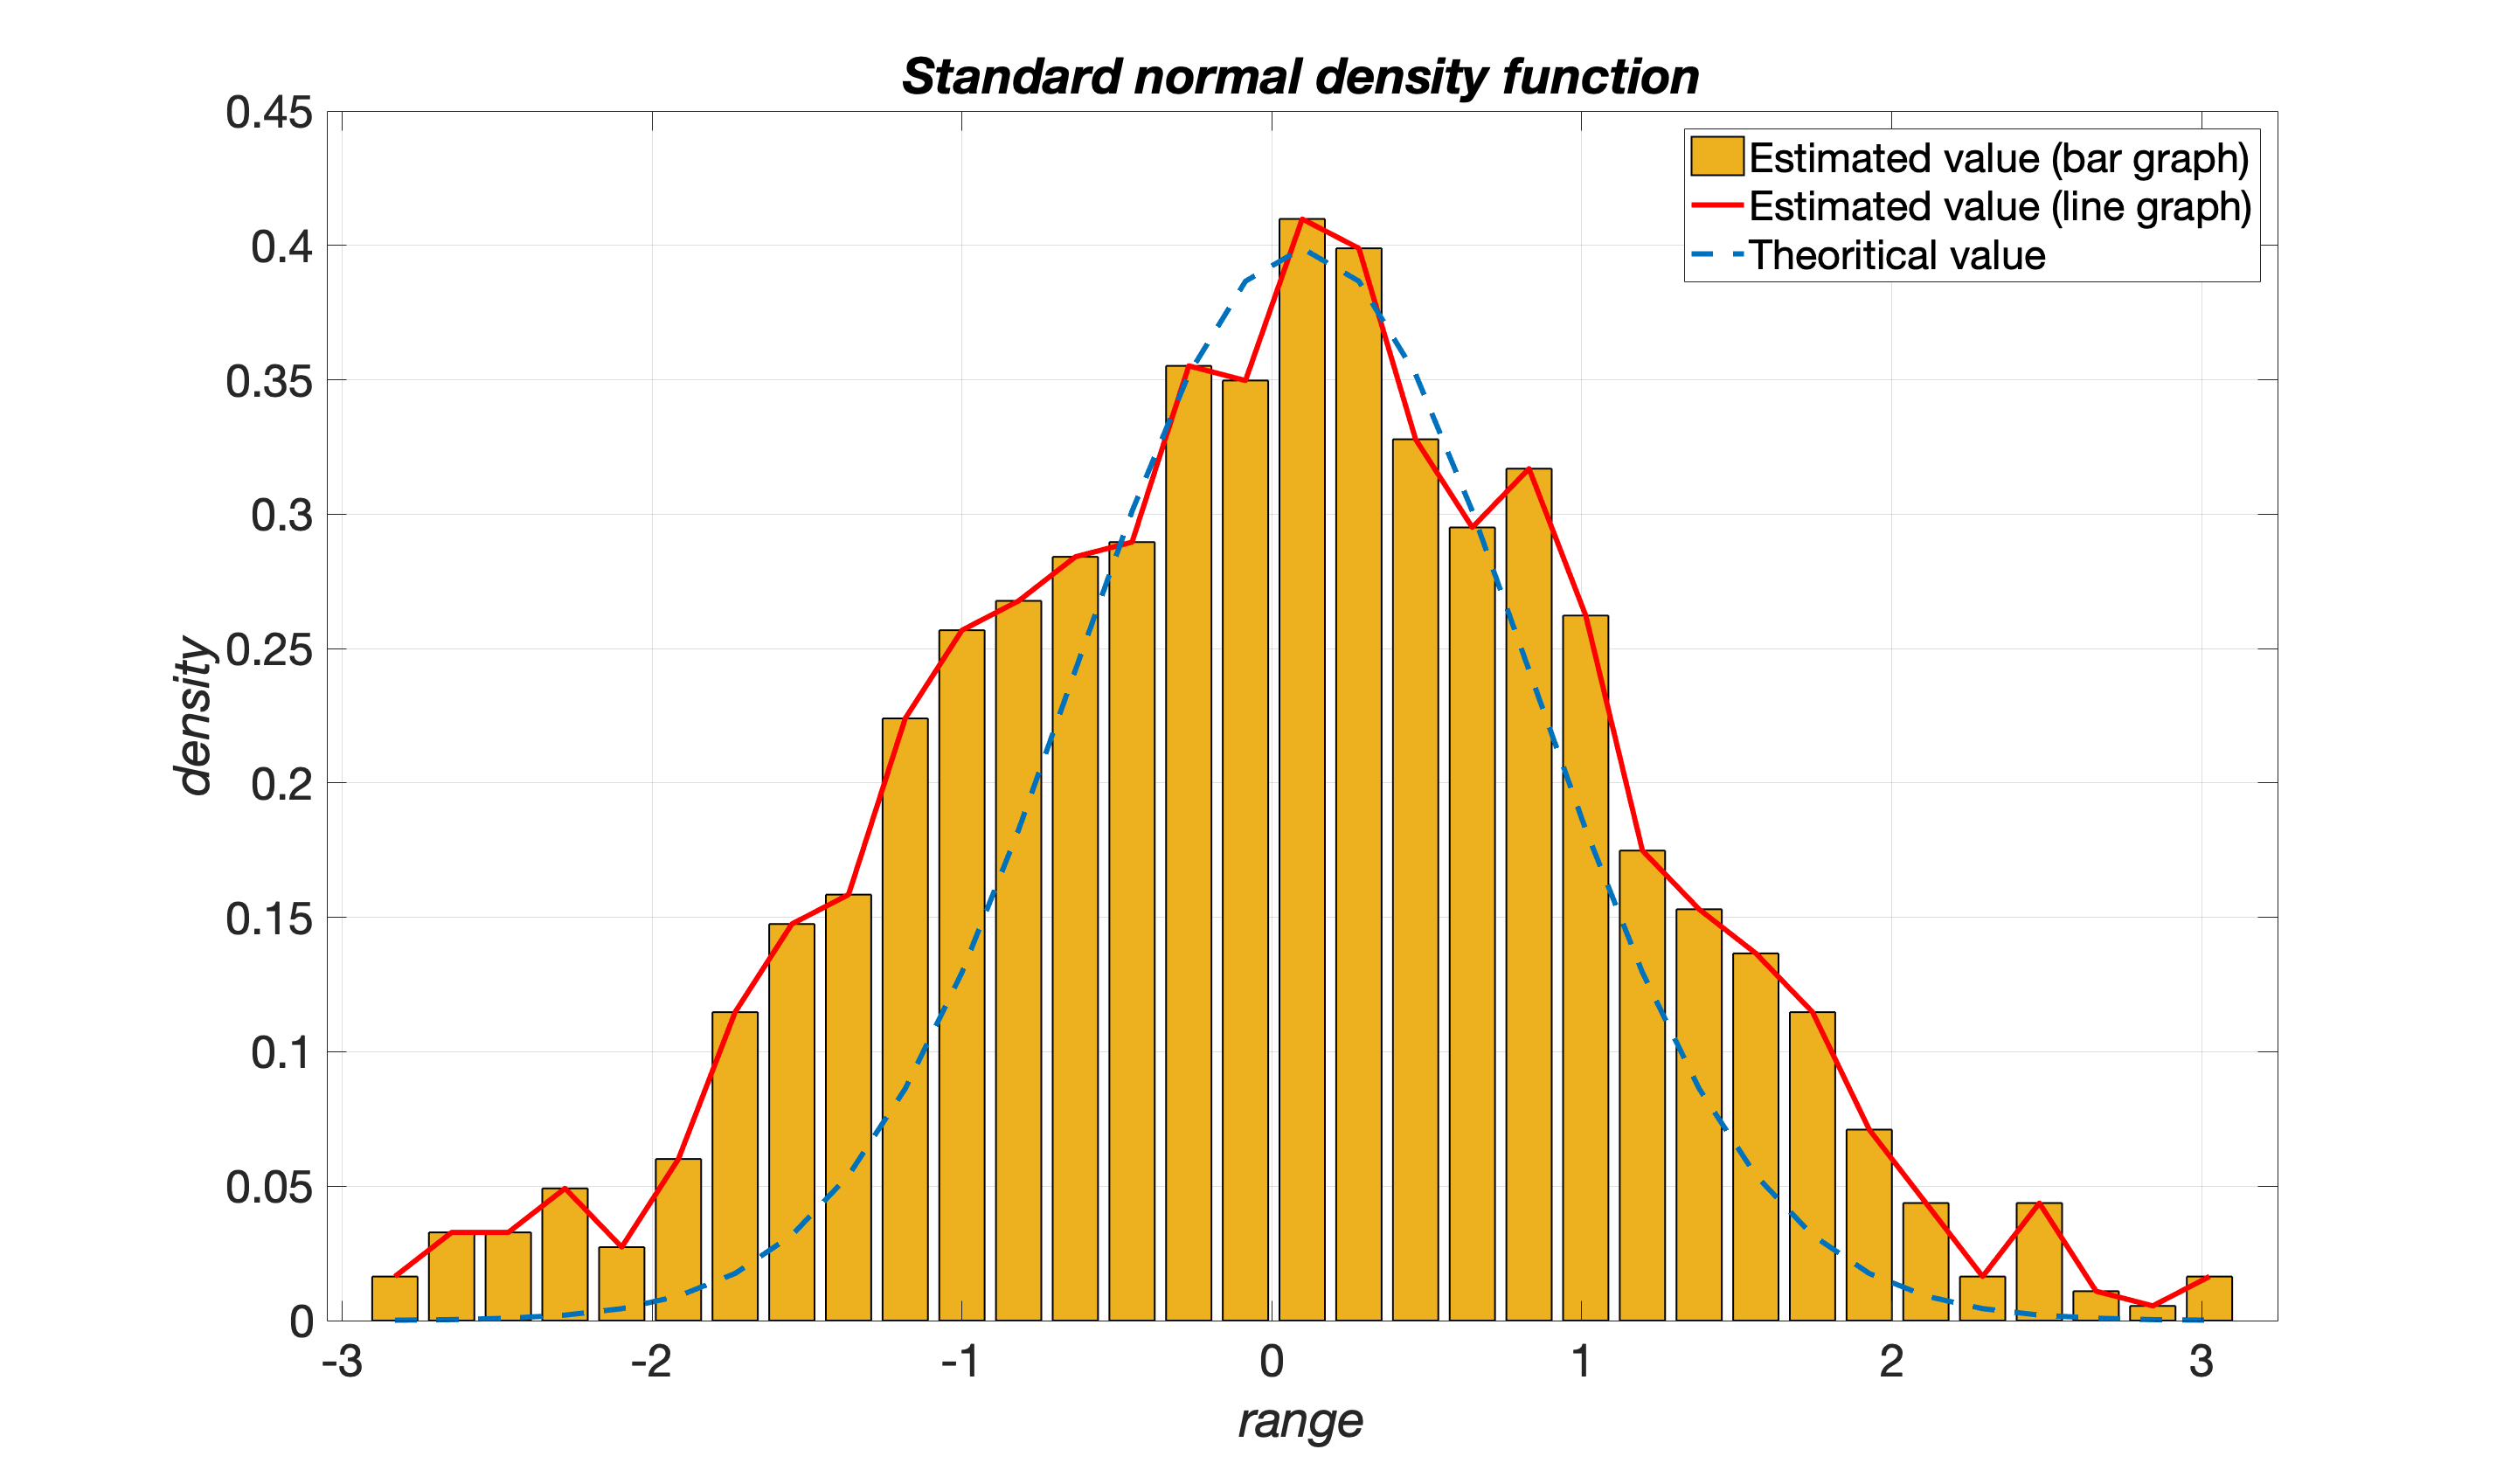
\includegraphics[scale=0.16]{ass1_1.png}}
\caption{Standard normal density function}
\label{Standard normal density function}
\end{figure}
\noindent The output below shows the comparison of the theoretical value (from section 1.1.) and the estimated value (from the MATLAB code) of the mean and variances.
\begin{figure}[H]
\centering
{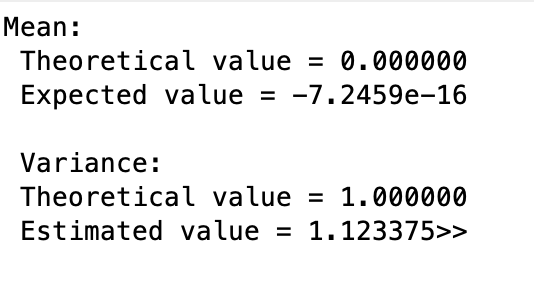
\includegraphics[scale=0.63]{ass1_2.png}}
\end{figure}
\noindent \textbf{Inference:} We can infer that the theoretical value almost coincides with the estimated value. We can observe that the estimated function is very much close to the Gaussian bell obtained by the theoretical density function.

%%%%%%%%%%% code 2 %%%%%


\section{ Exponential distribution } \label{ Exponential distribution }
\noindent \textbf{Task:} Load the on [0, 1] uniformly distributed random sequence from \texttt{dat1\_1} and transform it as explained in section 1.2 with $\alpha = 1/2.$ Calculate the sample mean and sample variance of the transformed sequence and compare the results with the theoretical values from section 1.2. Show the in section 1.2 calculated and via \texttt{density} estimated density function of the transformed random sequence in a figure. 

\noindent \textbf{Solution:}
\noindent \texttt{density} A uniformly distributed random sequence from \texttt{dat1\_1} is loaded and transformed  as explained in section 1.2 with $\alpha = 1/2.$  .The uniform density function as well as the normal density function is estimated by using the function \texttt{hist}. Line graph of both theoretical and estimated values are plotted in-order to compare the two. 

\noindent \textbf{MATLAB code:}
\lstinputlisting{assignment2_2.m}

\noindent \textbf{Output:}
\noindent The output after execution of the code is shown below. The estimated value is shown using both, bar and line graphs. While, dotted line shows the theoretical value.
\begin{figure}[H]
\centering
{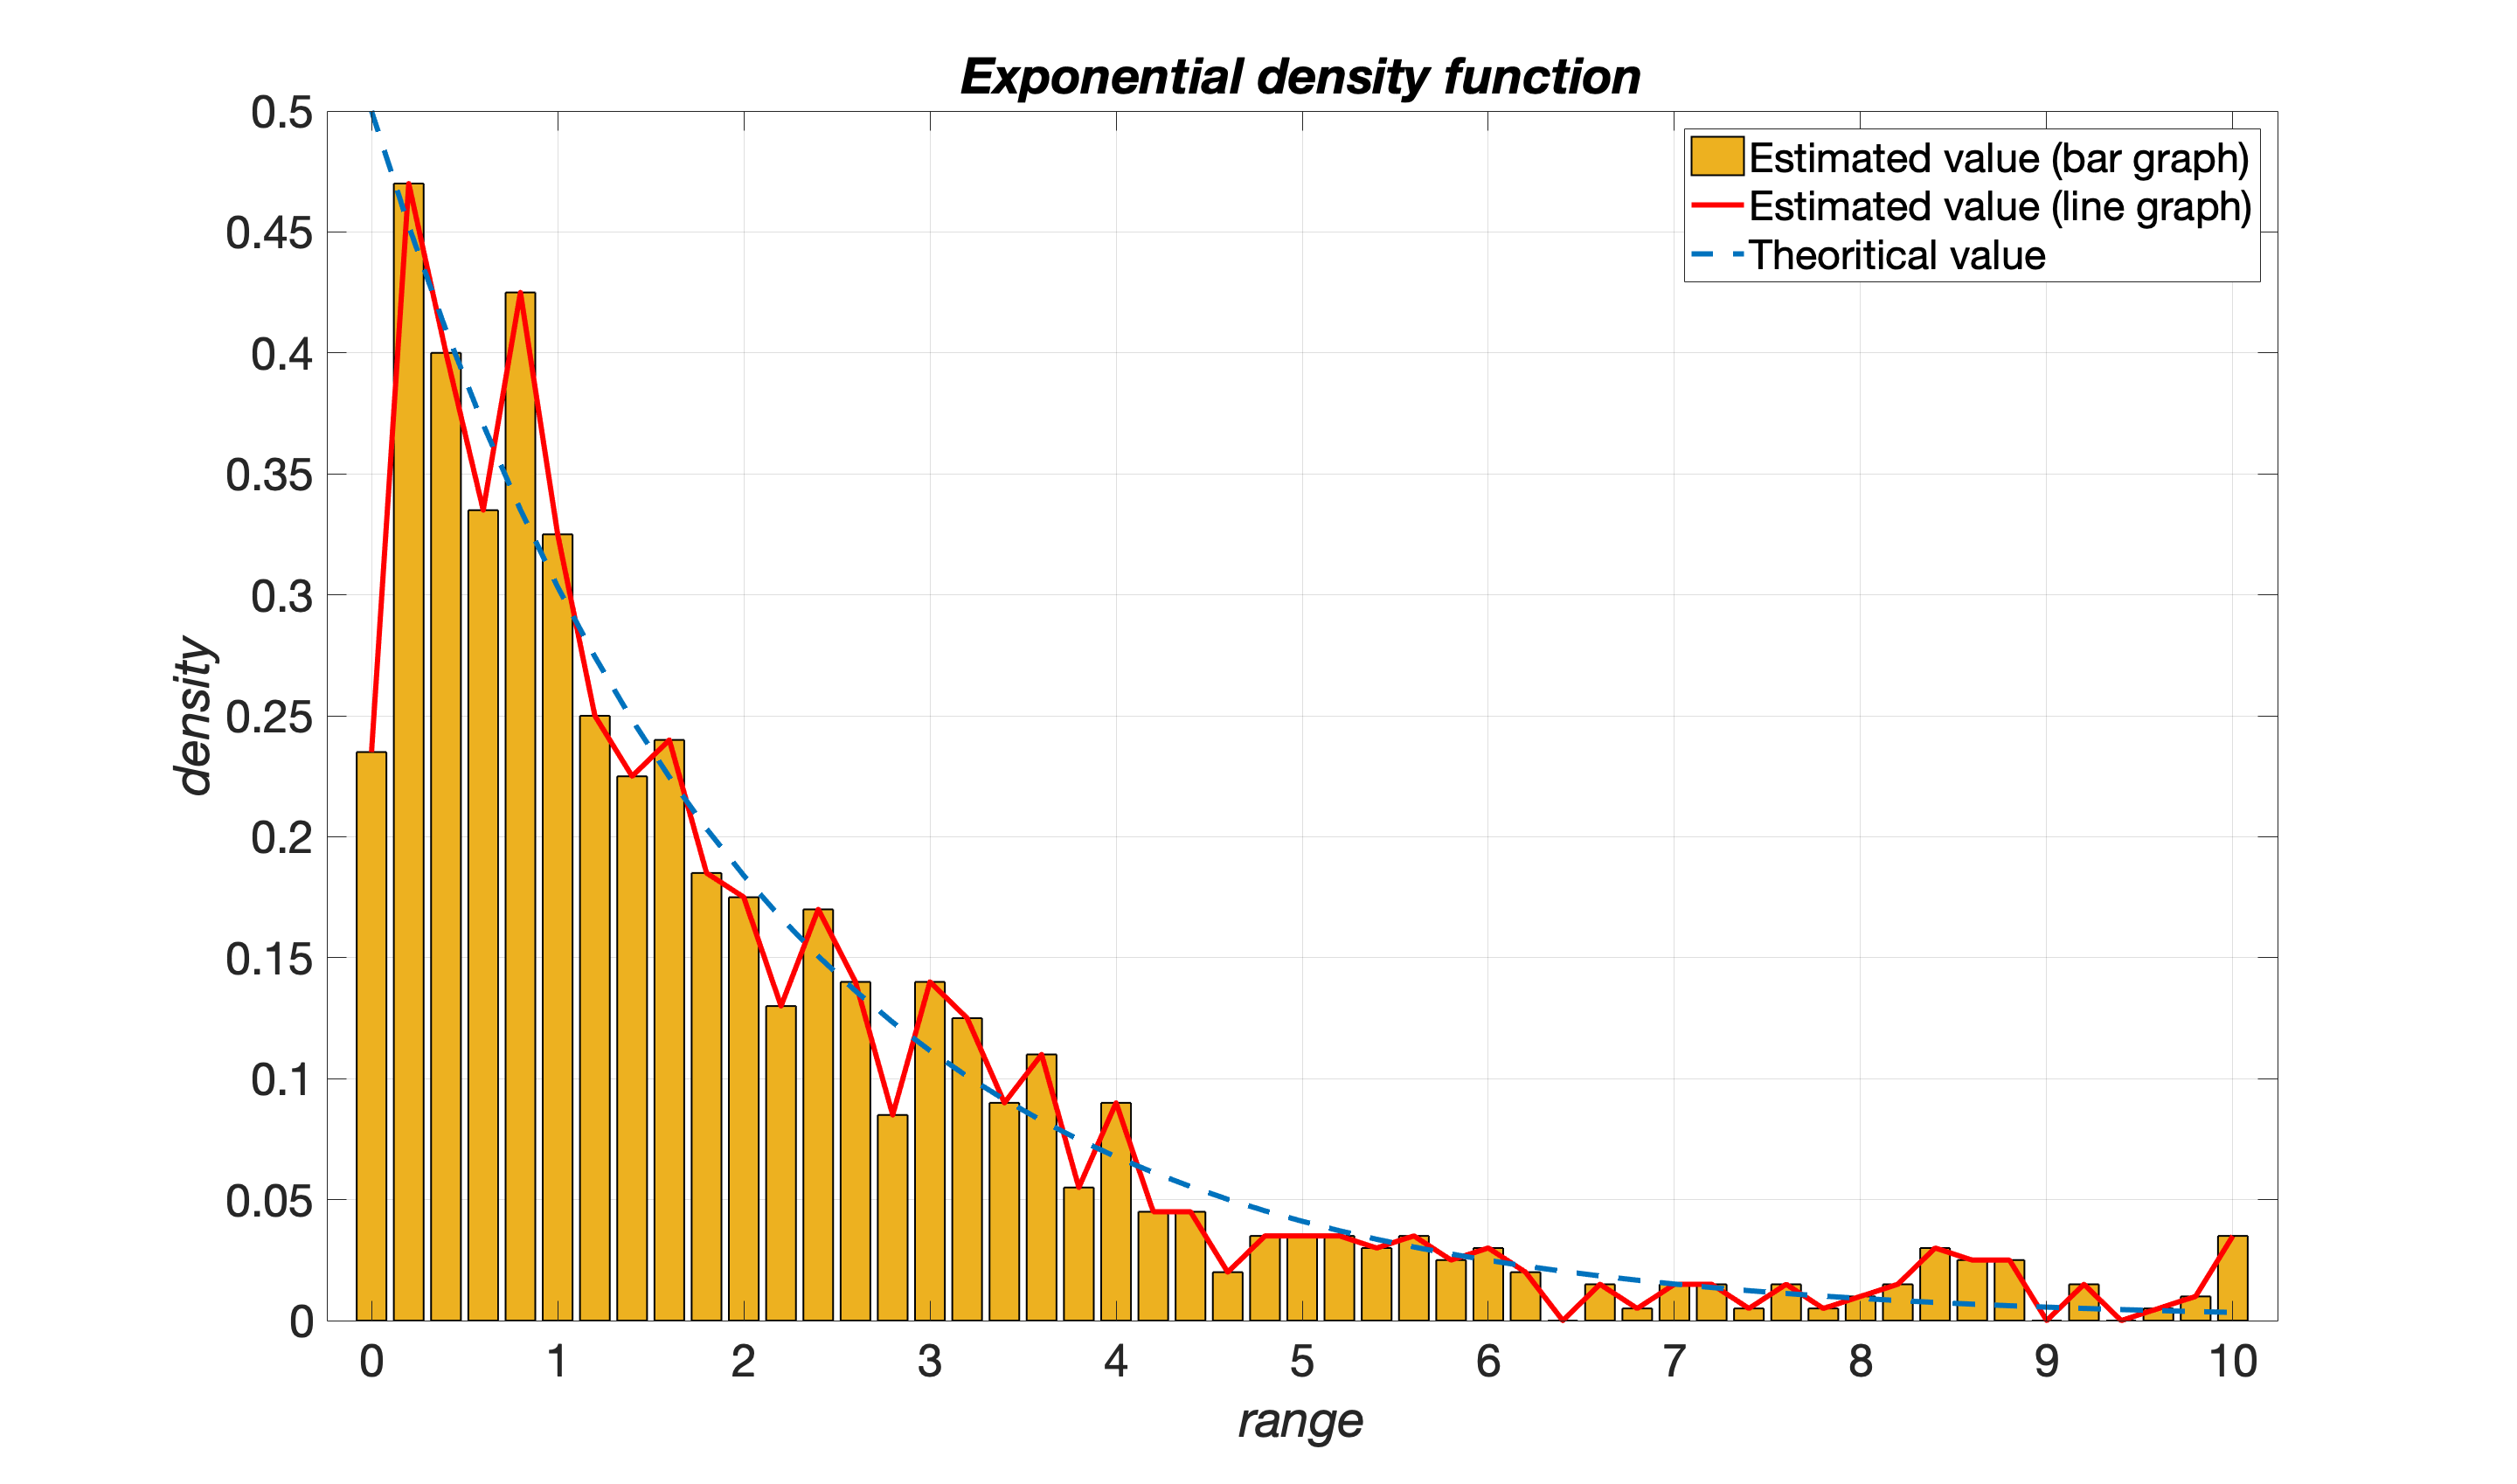
\includegraphics[scale=0.16]{ass2_1.png}}
\caption{Exponential density function}
\label{Exponential density function}
\end{figure}


\noindent The output below shows the comparison of the theoretical value (from section 1.2) and the estimated value (from the MATLAB code) of the mean and variances.
\begin{figure}[H]
\centering
{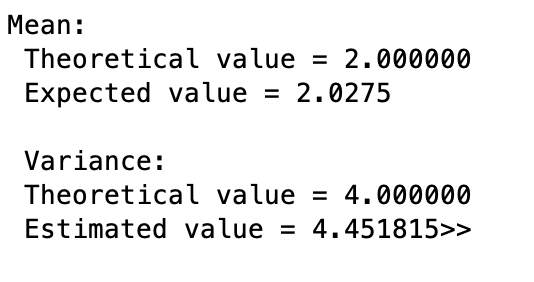
\includegraphics[scale=0.63]{ass2_2.png}}
\end{figure}

\noindent \textbf{Inference:} We can infer that the theoretical value almost coincides with the estimated value. From the output, we can observe small change in the values which is due to the length of the sample.
%%%%%%%%%%%%%%% code 3 %%%%%


\section{ Sum of random numbers  } \label{ Sum of random numbers }
\noindent \textbf{Task:} Generate two on [0, 1] uniformly distributed random sequences of the length 1000 after setting the initial value to 0. Save both random sequences in  \texttt{dat2\_1}.   Then add the two sequences element-by-element. Calculate the sample mean and sample variance of the sum and compare the results with the theoretical values from section 2.1.3. Display the in section 2.1.3 calculated and via \texttt{density} estimated density function in a diagram. 


\noindent \textbf{Solution:} First, two standard normal distributed random sequences of length 1000 were generated using the function \texttt{randn} and these were saved in \texttt{dat2\_1.}  .The two random sequences from \texttt{dat2\_1} were added element-by-element and this density function of the resulting product was calculated.


\noindent \textbf{MATLAB code:}
\lstinputlisting{assignment2_3.m}


\noindent \textbf{Output:}
\noindent The output after execution of the code is shown below. The estimated value is shown using both, bar and line graphs. While, dotted line shows the theoretical value.
\begin{figure}[H]
\centering
{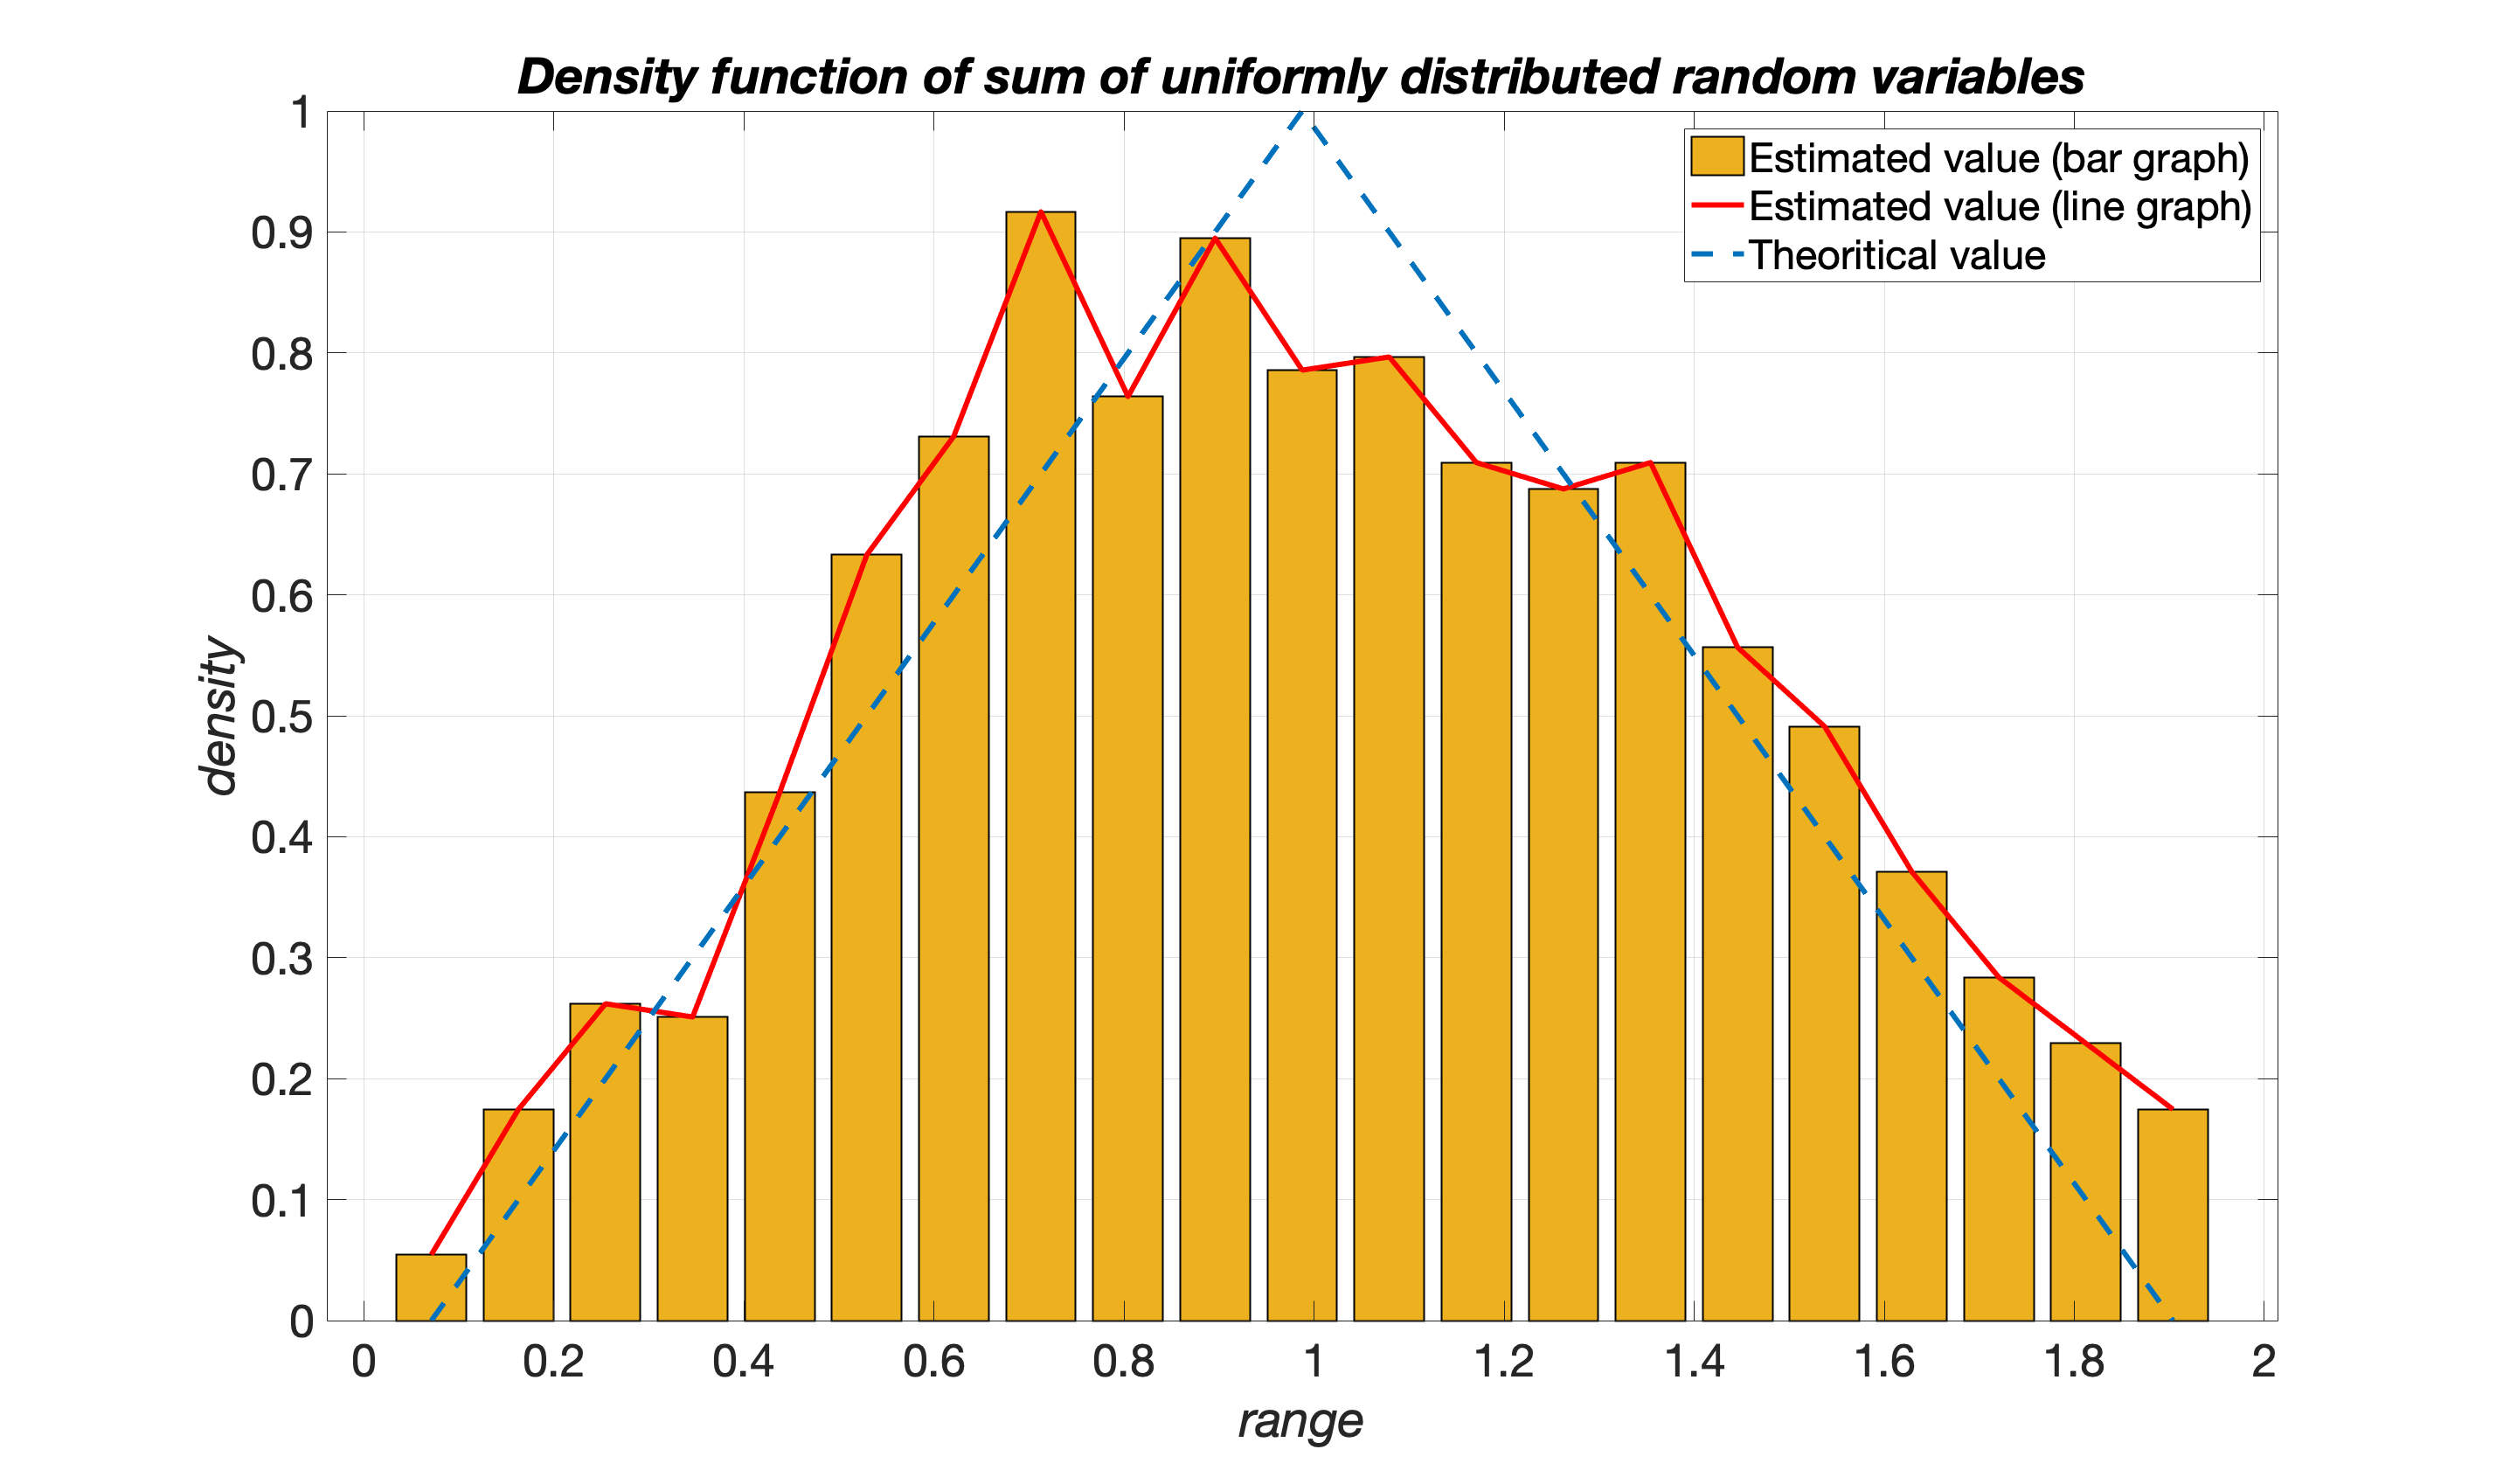
\includegraphics[scale=0.16]{ass3_1.png}}
\caption{Density function of sum of uniformly distributed random variables}
\label{Density function of sum of uniformly distributed random variables}
\end{figure}

\noindent The output below shows the comparison of the theoretical value (from section 1.3) and the estimated value (from the MATLAB code) of the mean and variances of the sum of random sequences.
\begin{figure}[H]
\centering
{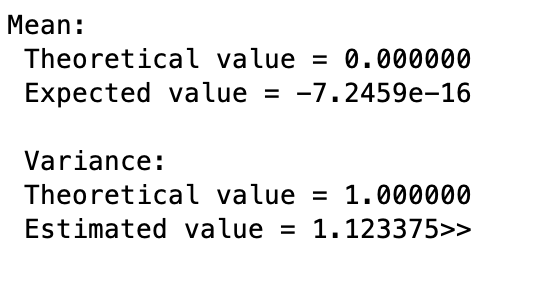
\includegraphics[scale=0.63]{ass3_2.png}}
\end{figure}

\noindent \textbf{Inference:} We can infer that the theoretical value almost coincides with the estimated value. The small variation in the value is due to the sample length.


%%%%%%%% code 4 %%%%%


\section{ Product of random numbers } \label{ Product of random numbers }
\noindent \textbf{Task:} Multiply both on [0, 1] uniformly distributed random sequences from \texttt{ dat2\_1} element by element. Calculate the sample mean and sample variance of the product and compare the results with the theoretical values derived in section 1.4. Depict the in section 1.4 calculated and via density estimated density function in a figure. 

\noindent \textbf{Solution:} The two random sequences from \texttt{dat2\_1} were multiplied element-by-element and this density function of the resulting product was calculated.

\noindent \textbf{MATLAB code:}
\lstinputlisting{assignment2_4.m}
\noindent \textbf{Output:} The output after execution of the code is shown below. The estimated value is shown using both, bar and line graphs. While, dotted line shows the theoretical value.

\begin{figure}[H]
\centering
{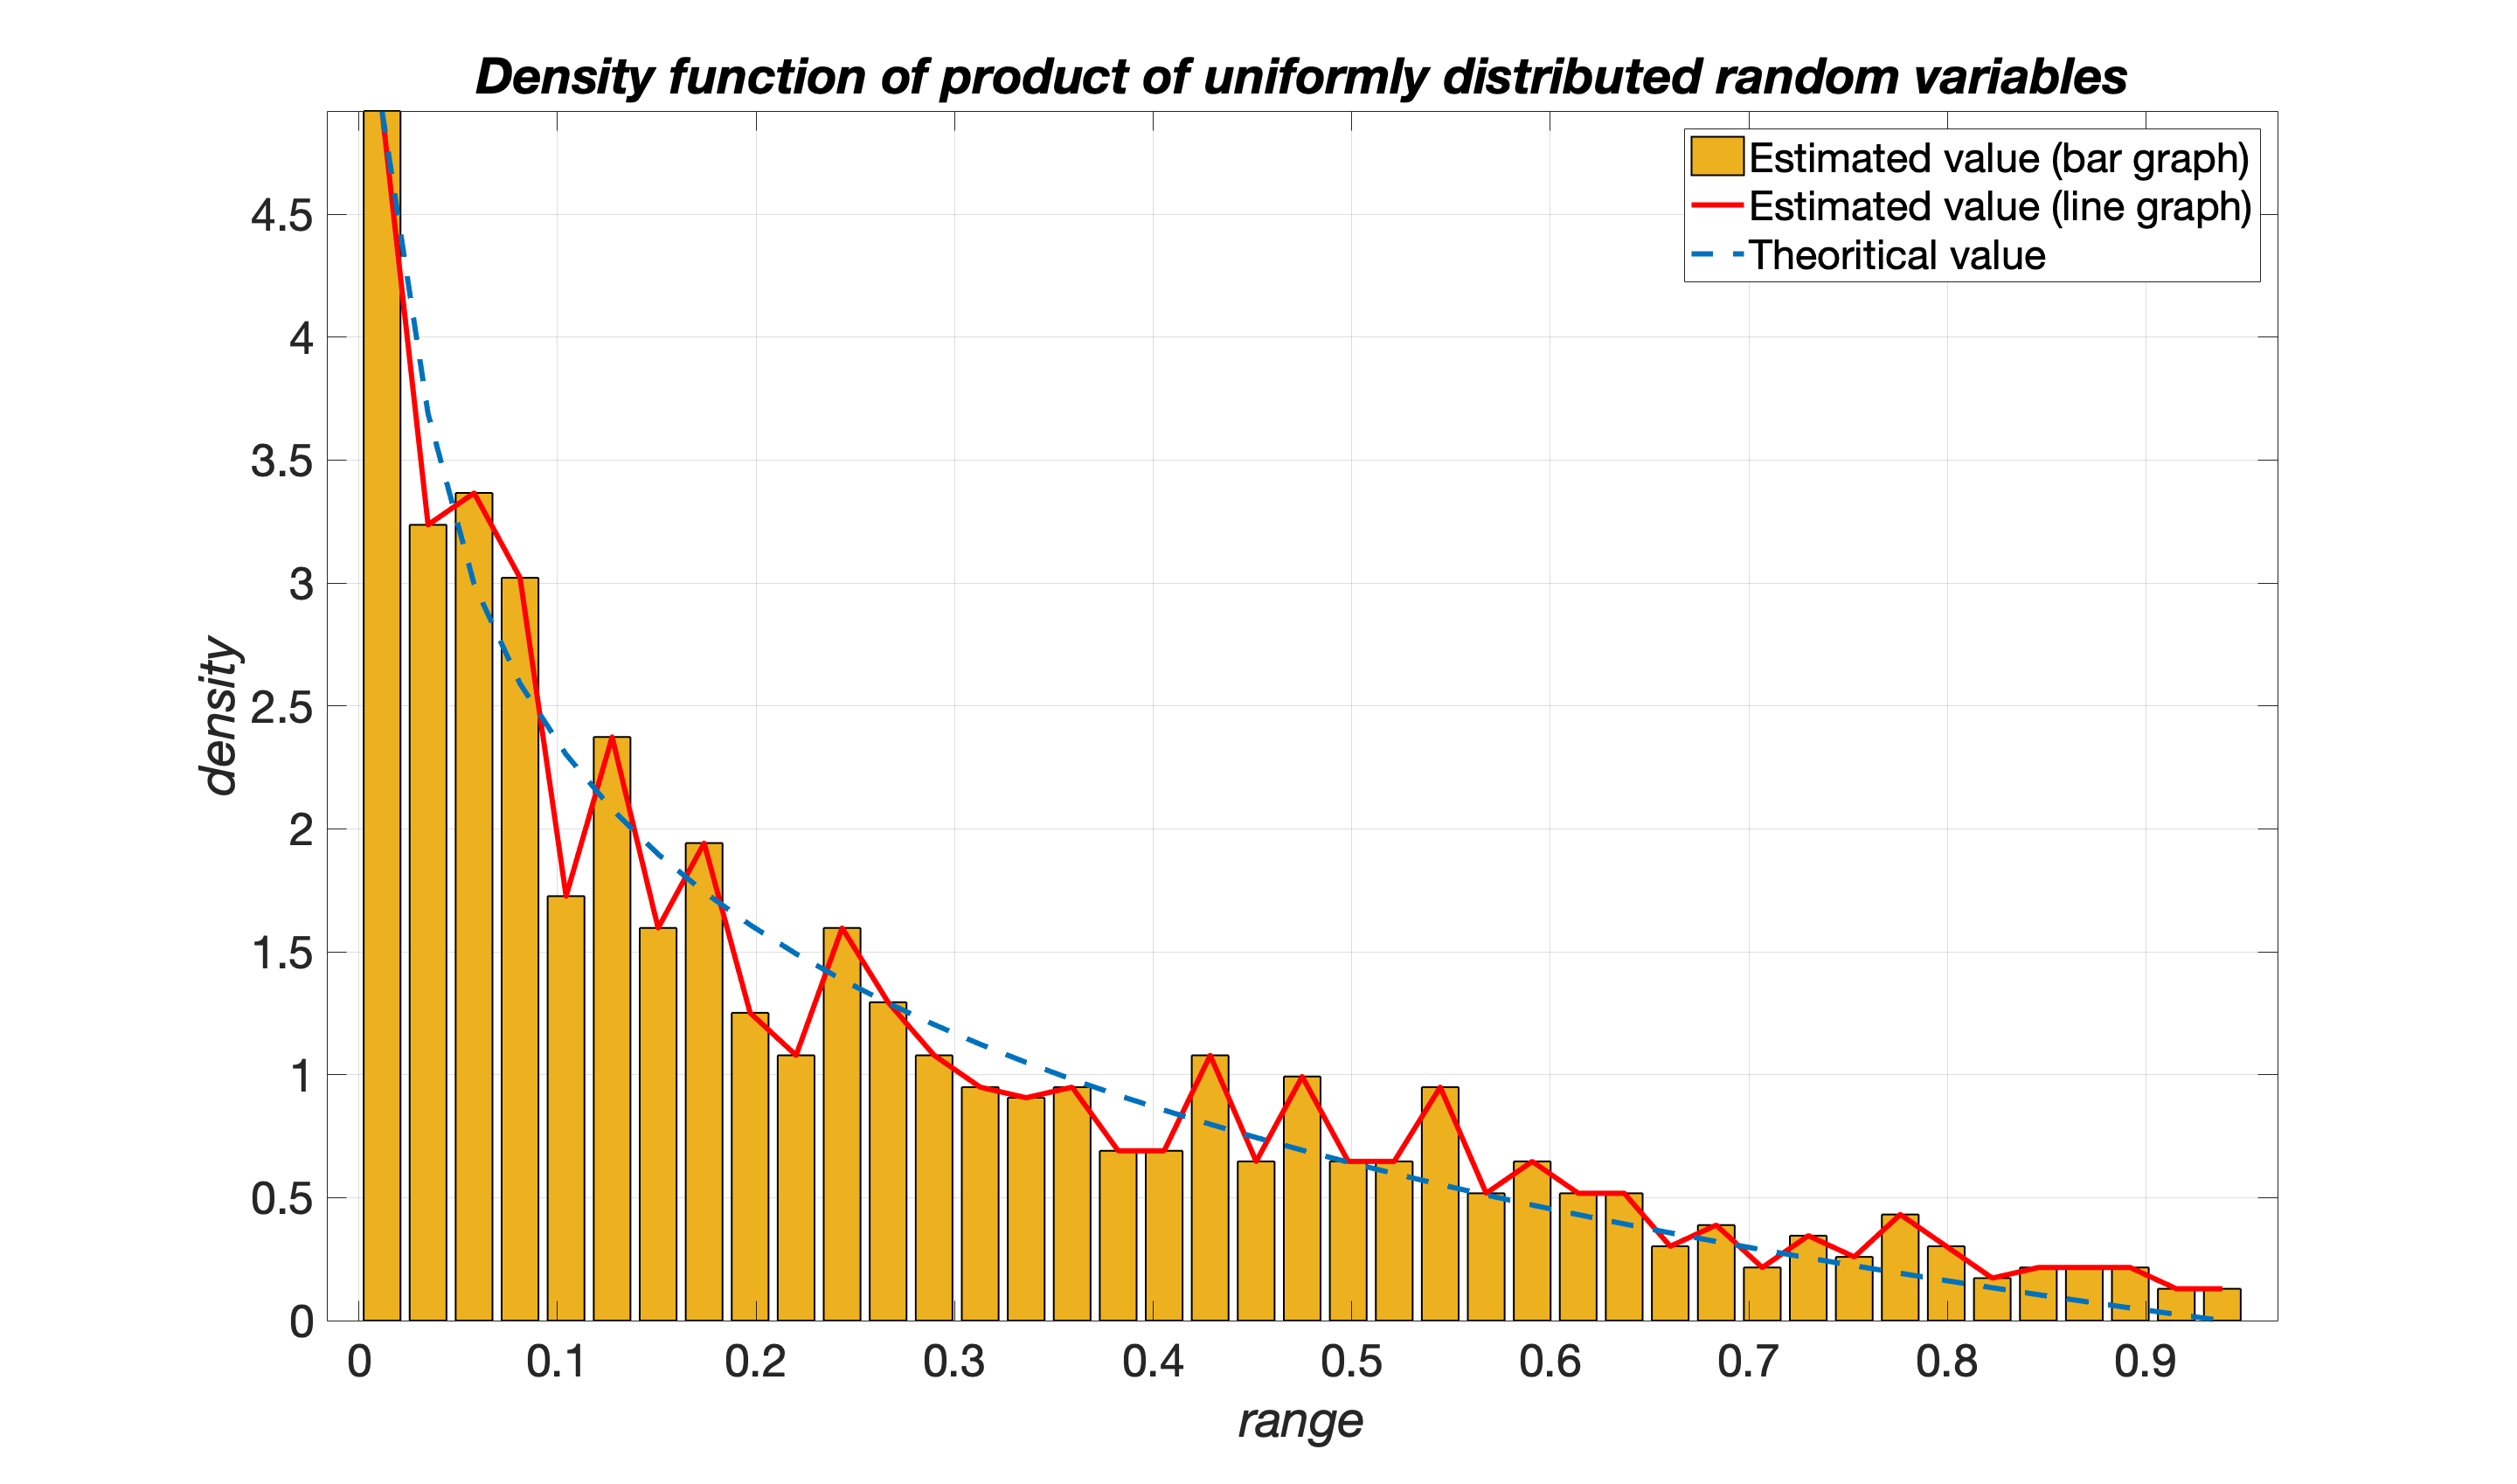
\includegraphics[scale=0.16]{ass4_1.png}}
\caption{Density function of product of uniformly distributed random variables}
\label{Density function of product of uniformly distributed random variables}
\end{figure}

\noindent he output below shows the comparison of the theoretical value (from section 1.4) and the estimated value (from the MATLAB code) of the mean and variances of the product of random sequences.

\begin{figure}[H]
\centering
{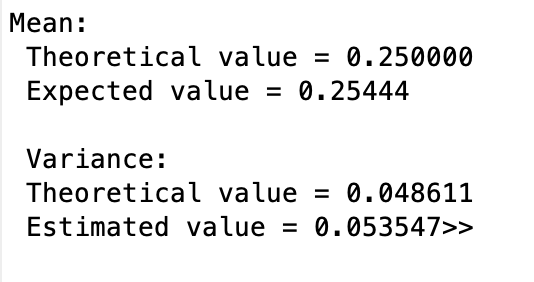
\includegraphics[scale=0.63]{ass4_2.png}}
\end{figure}

\noindent \textbf{Inference:} We can infer that the theoretical value almost coincides with the estimated value. The small variation in the value is due to the sample length. The theoretical curve depicts a smooth decaying curve whereas, the nature of the estimated curve is a decaying curve with many variations.
%%%%%%%%%%%  code 5  %%%%%


%\section{ $\chi$ distribution } \label{ $\chi$ distribution }
\section{$\chi^2$ -distribution } 
\noindent \textbf{Task:} Generate four standard normal distributed random sequences of the length 1000, where before the initial value has to be set to 0. Save the data in \texttt{dat2\_2.} Determine the sum of squares of the
four random sequences element-by-element. Calculate the sample mean and sample variance of
the sum and compare the results with the theoretical values obtained in section 1.5. Present the
in section 1.5 calculated and via density estimated \texttt{density} function in a diagram. 
 
 \noindent \textbf{Solution:} First, four standard normal distributed random sequences of length 1000 were generated using the function \texttt{randn} and these were saved in \texttt{dat2\_2.} The sum of squares of the four random sequences element-by-element was determined and the density function of it was calculated.
  
 \noindent \textbf{MATLAB code:}
\lstinputlisting{assignment2_5.m}

 \noindent \textbf{Output:}
 \noindent The output of the code is shown below. The estimated value is shown using both, bar and line graphs. While, dotted line shows the theoretical value. 
\begin{figure}[H]
\centering
{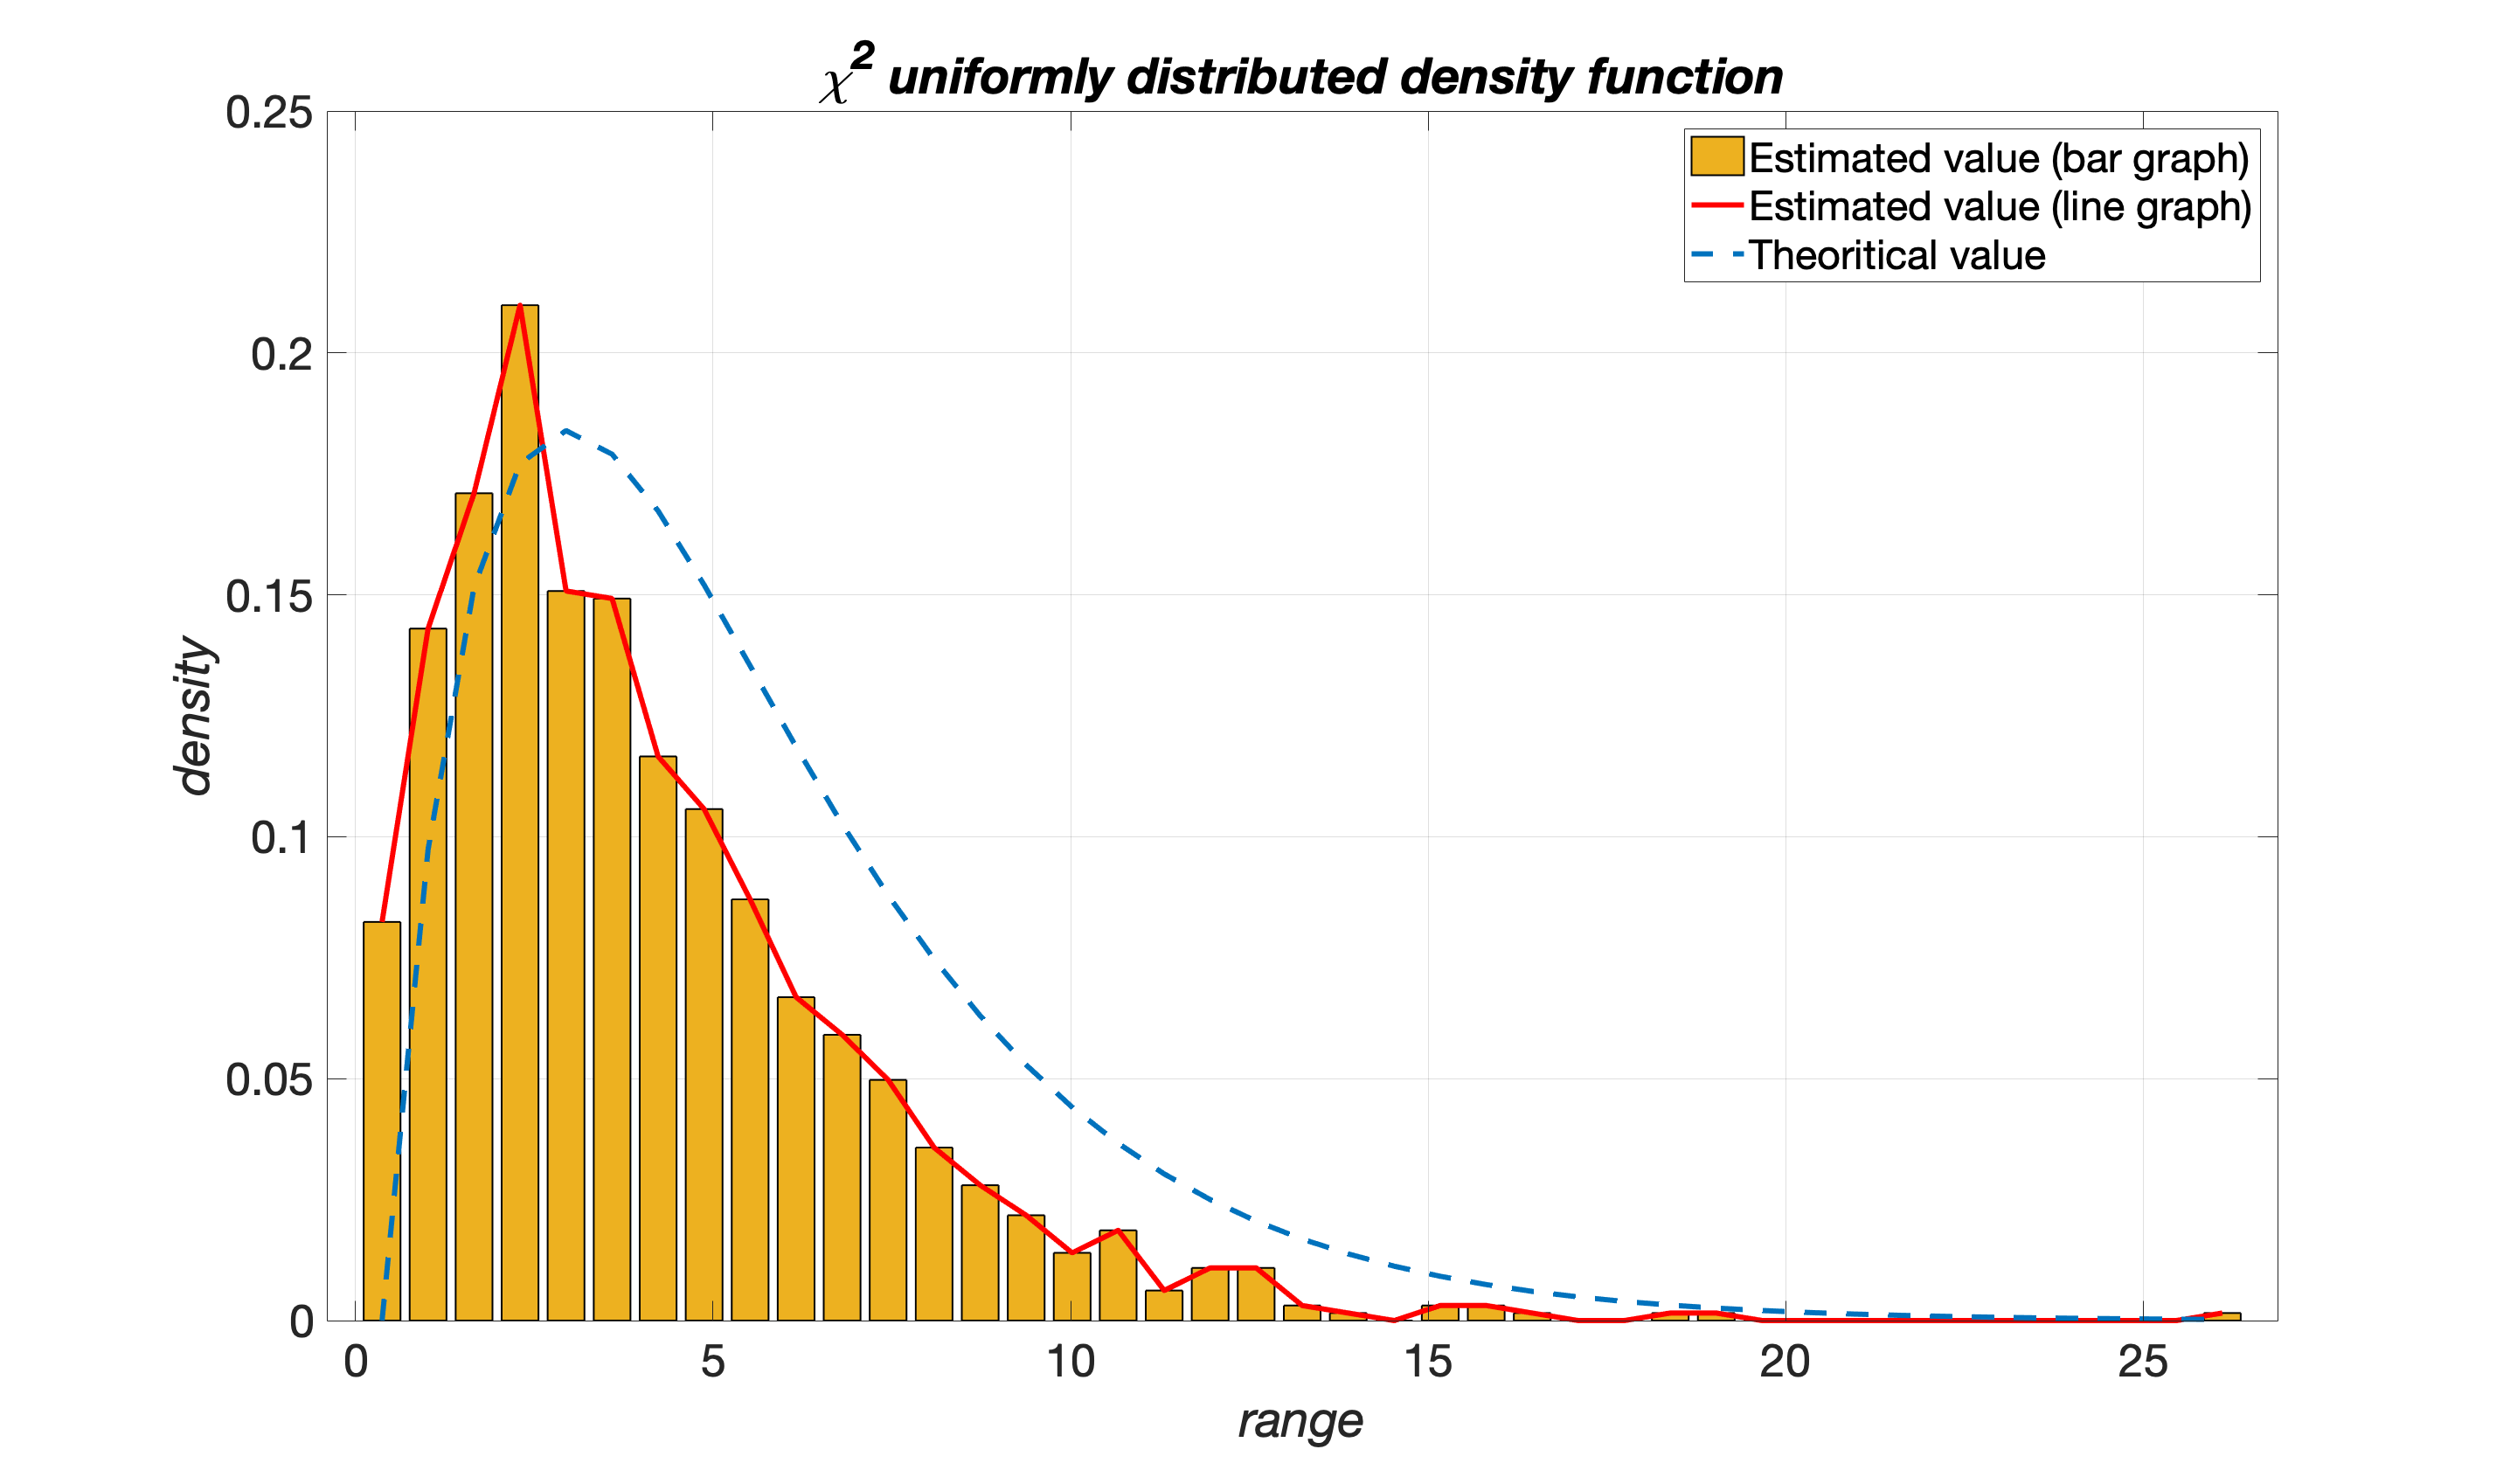
\includegraphics[scale=0.16]{ass5_1.png}}
\caption{$\chi^2$ uniformly distributed density function }
%\label{$\chi^2$ -distribution}
\end{figure}
\noindent The output below shows the comparison of the theoretical value (from section 1.5) and the estimated value (from the MATLAB code) of the mean and variances of the sum of squares of the four random sequences.
\begin{figure}[H]
\centering
{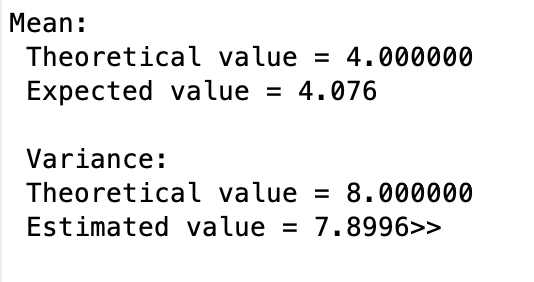
\includegraphics[scale=0.63]{ass5_2.png}}
\end{figure}

\noindent \textbf{Inference:} We can infer that the theoretical value almost coincides with the estimated value. The small variation in the value is due to the sample length.


%%%%%% code 6 %%%%%%

\section{ Normal distribution from uniform distribution  }  \label{ Normal distribution from uniform distribution }
\noindent \textbf{Task:} Now use again \texttt{dat2\_1} containing two on [0, 1] uniformly distributed random sequences. Build \textbf{y1} as explained in section 1.6. Calculate the sample mean and sample variance of \textbf{y1} and compare the results with the theoretical values determined in section 2.1.6. Show the in section 1.6 calculated and via \texttt{density} estimated density function in a figure. 


\noindent \textbf{Solution:} \texttt{dat2\_1} was loaded as mentioned in the task. \texttt{y1} was considered to be the first column of \texttt{dat2\_1}, i.e, \texttt{random\_Seq\_1}. The estimated density of \texttt{y1} was calculated by the function called \texttt{density}.

\noindent \textbf{MATLAB code:} 
\lstinputlisting{assignment2_6.m}

\noindent \textbf{Output:} The output of the code is shown below. The estimated value is shown using both, bar and line graphs. While, dotted line shows the theoretical value.
\begin{figure}[H]
\centering
{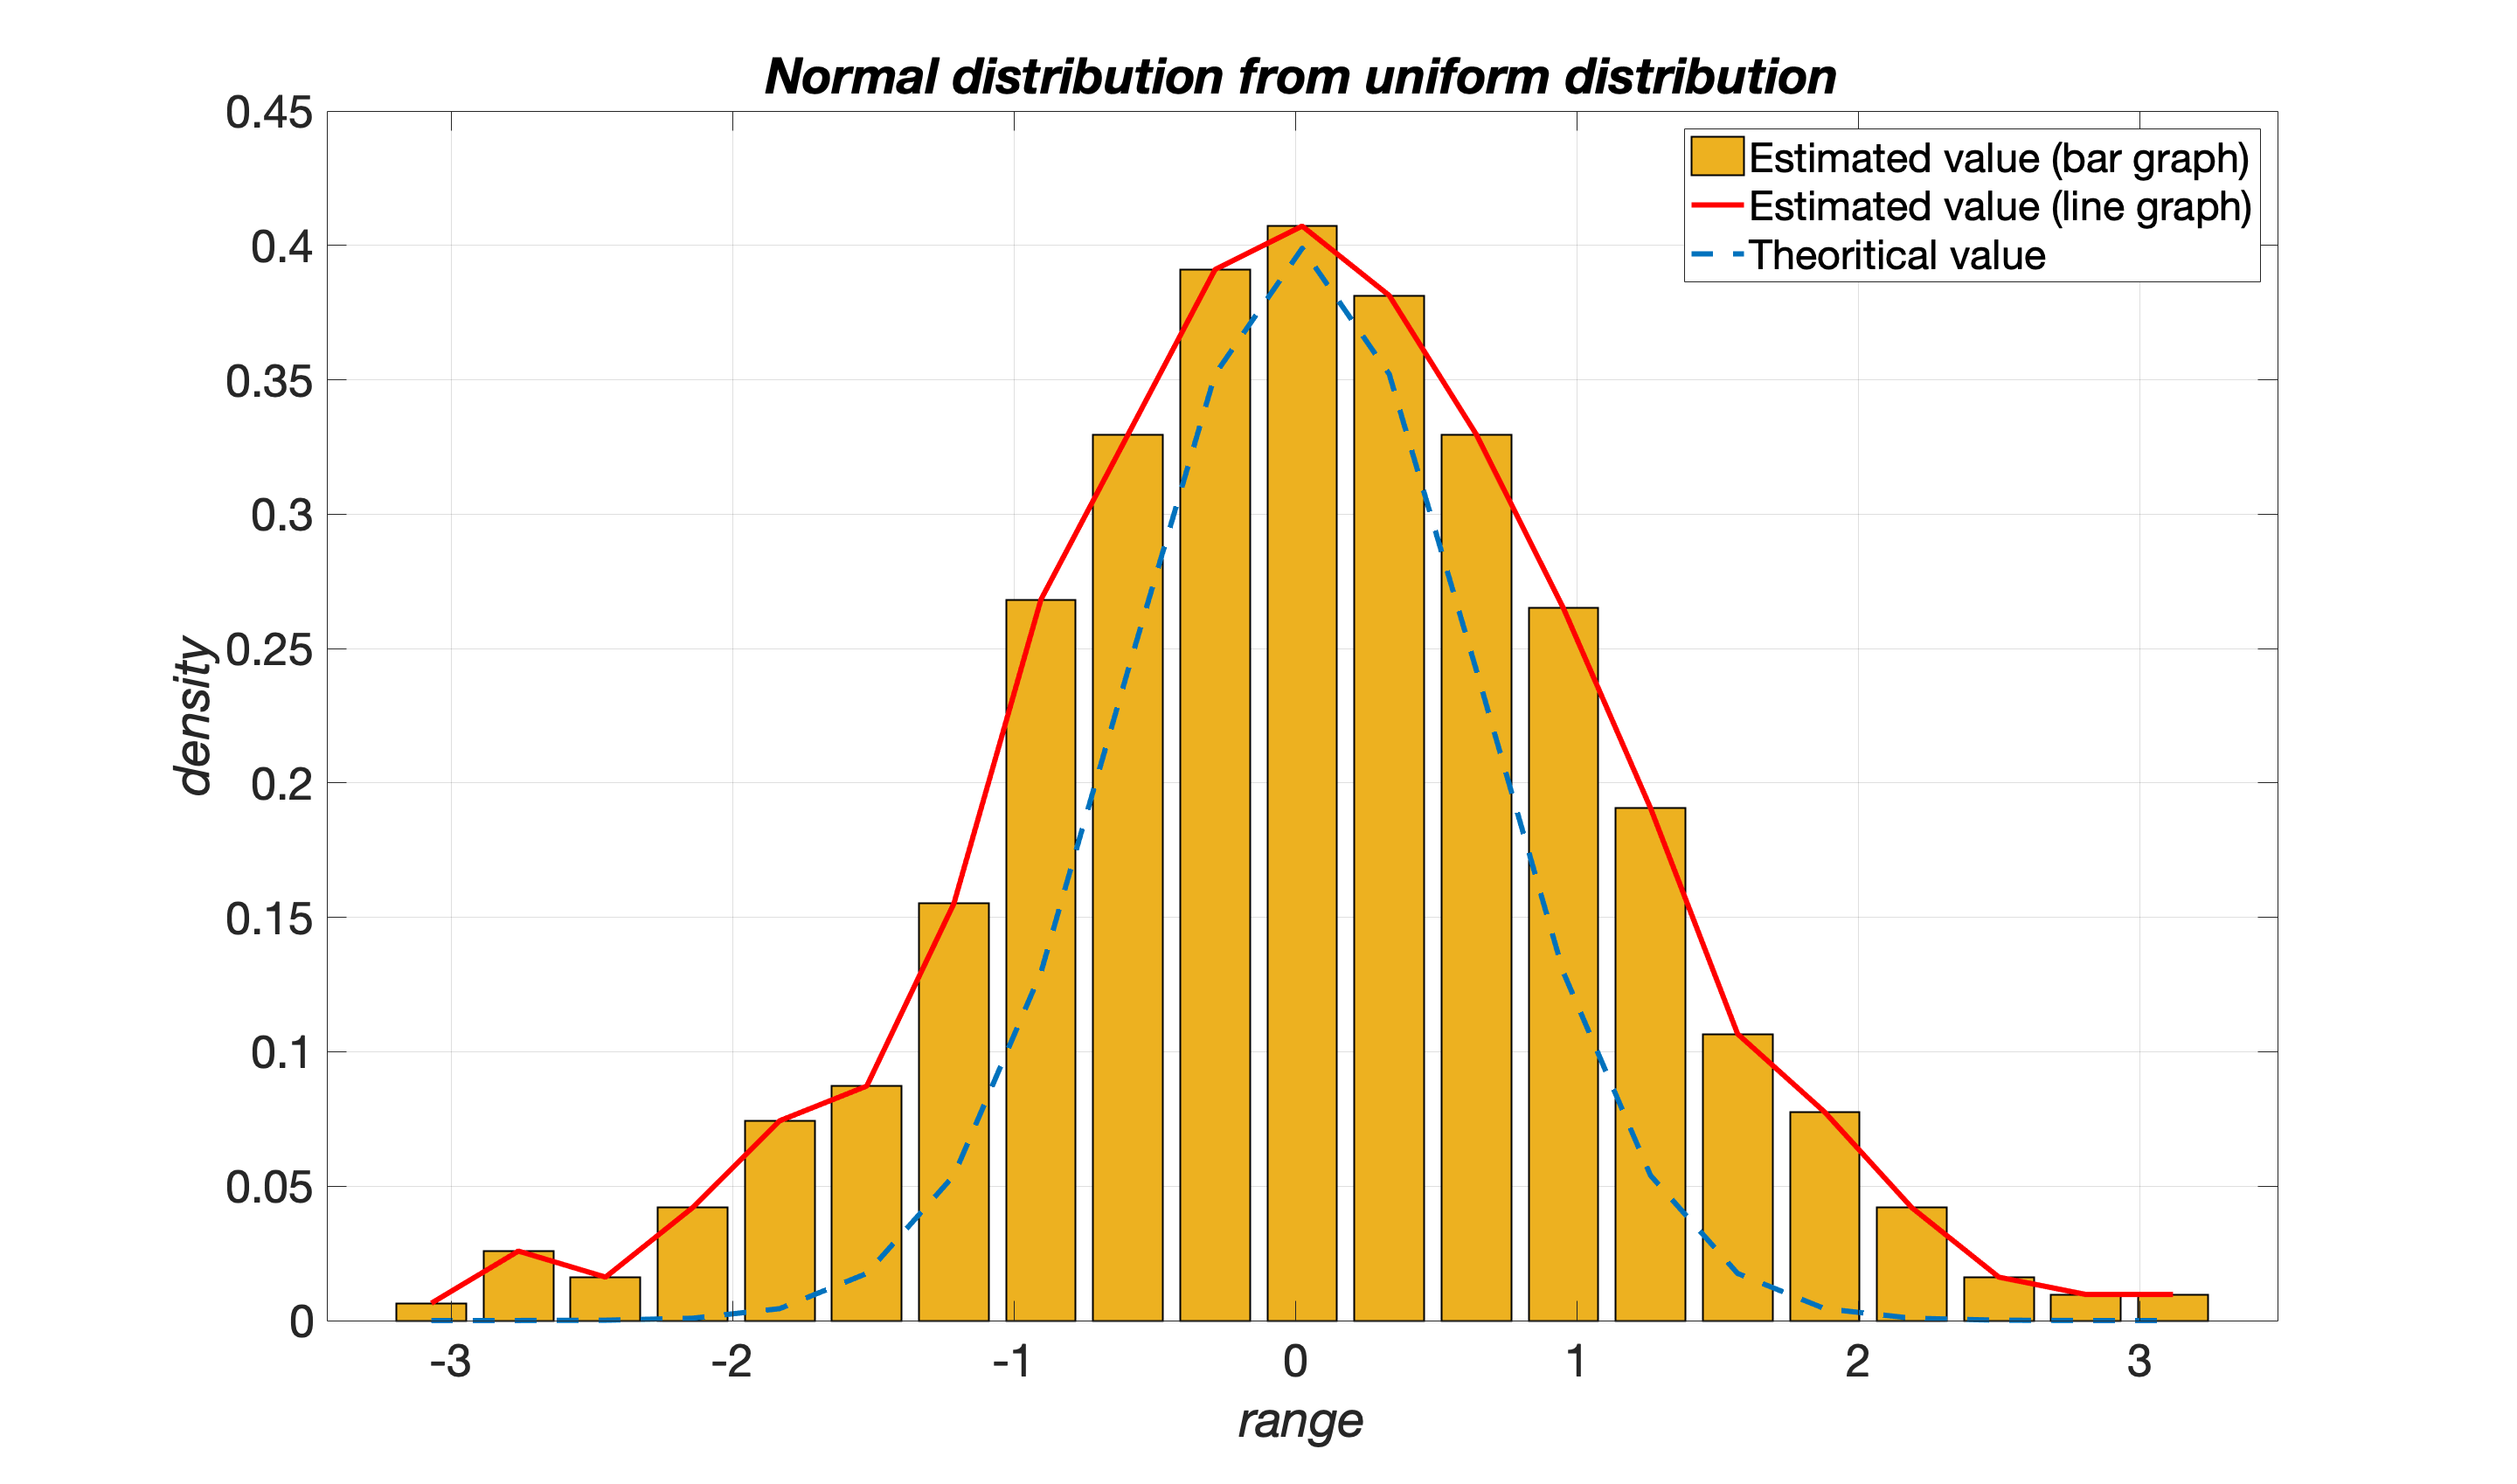
\includegraphics[scale=0.16]{ass6_1.png}}
\caption{Normal distribution from uniform distribution }
\label{Normal distribution from uniform distribution }
\end{figure}

\noindent The output below shows the comparison of the theoretical value (from section 1.6) and the estimated value (from the MATLAB code) of the mean and variances of the transformed y1.
\begin{figure}[H]
\centering
{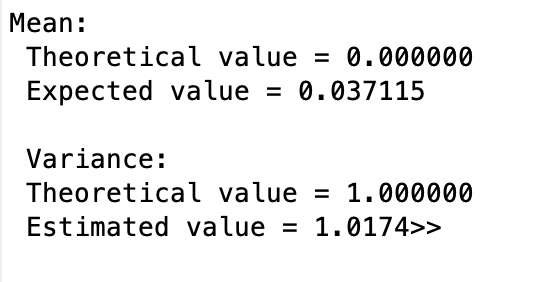
\includegraphics[scale=0.63]{ass6_2.png}}
\end{figure}

\noindent \textbf{Inference:} We can infer that the theoretical value almost coincides with the estimated value. The estimated graph of \texttt{y1} shows a normal uniformly distributed curve, whereas the obtained theoretical graph is a bivariate density function curve with mean as 0 and variance as 1.
